\documentclass{article}

\usepackage[english]{babel}
\usepackage[utf8]{inputenc}
\usepackage{rotating}
\usepackage[top=2.5cm, left=3cm, right=3cm, bottom=4.0cm]{geometry}
\usepackage[toc,page]{appendix}

\usepackage{color, soul}
\usepackage{amsmath}

\usepackage[table]{xcolor}


\newcommand{\tablespace}{\\[1.25mm]}
\newcommand\Tstrut{\rule{0pt}{2.6ex}}
\newcommand\tstrut{\rule{0pt}{2.0ex}}
\newcommand\Bstrut{\rule[-0.9ex]{0pt}{0pt}}

\title{CO395 - Machine Learning Coursework 2}
\author{
    Padmanaba Srinivasan \\
    \texttt{01191525}
    \and
    Keerthanen Ravichandran \\
    \texttt{01195170}
    \and
    Harrison Ankers \\
    \texttt{01211208}
    \and
    Tze Hei Tang \\
    \texttt{01221240}
}
\date{\today}

\begin{document}
\maketitle
\newpage
\tableofcontents
\newpage

\section{Part 2}
\subsection{Q2.1: Implementing the forward model of the ABB IRB 120}
\subsubsection{Creating the Neural Network model using Keras}
Using Keras to create a Neural Network Model is trivial and can be accomplished in a few lines of code as in figure \ref{fig:keras_nn_code}.
\begin{figure}[h]
    \centering
    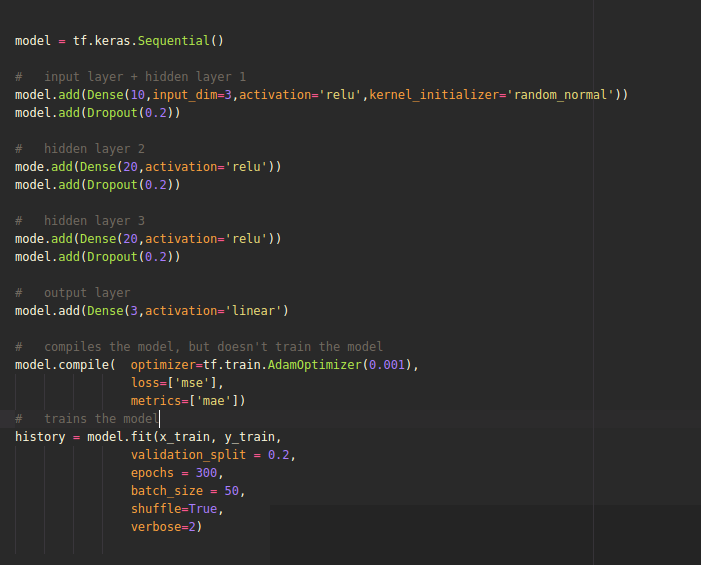
\includegraphics[scale=0.5]{figure/basic_model.png}
    \caption{Basic neural network using Keras}
    \label{fig:keras_nn_code}
\end{figure}
\\

This model is created with 3 hidden layers, each with 10, 20, and 20 neurons respectively. All layers use $Relu$ as the neuron activation function, with a dropout rate of 0.2. There are three input nodes and three linear output nodes. All the nodes are initialised using a Random Normal method. 

An adaptive learning rate method called $Adam$ has been implemented with an input rate of 0.001; this method was chosen as it is computationally efficient (which becomes more relevant when optimising hyperparameters) and memory efficient. The Loss Function and Validation Metric are Mean Squared Error (MSE) and Mean Absolute Error (MAE) respectively. MSE and MAE were chosen as the problem is one of regression and these are well suited to this. Furthermore, MAE is more robust to outliers than MSE and using this yielded some improvement in the Neural Network's performance. 

Finally, a validation split of 20\% was decided upon along with 300 Epochs to ensure there are sufficient number of trials for the network to learn and come to a stable point where further training yields no more benefit. A batch size of 50 was used. The metrics were determined by looking at how regression problems with Neural Networks are usually solved and with intuition about the scope of the problem.

\newpage
\subsection{Q2.2: Evaluating the architecture}
\begin{figure}[h]
    \centering
    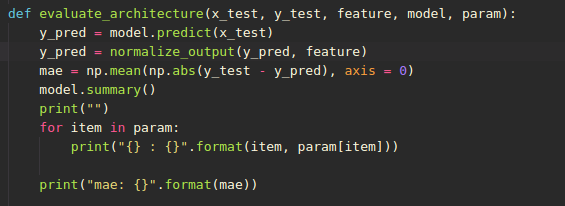
\includegraphics[scale=0.5]{figure/eval_arch.png}
    \caption{Evaluate architecture}
    \label{fig:eval_arch}
\end{figure}

The $evaluate \textunderscore architecture$ function (figure \ref{fig:eval_arch}) outputs the model structure (ie. number of layers and neurons etc.), the hyperparameters chosen for the model, and the accuracy on the test dataset.

\subsection{Q2.3: Fine tuning the architecture}
\subsubsection{Data preparation}

The initial dataset was split into a training set, validation set and test set in a ratio of 6/2/2. The entire dataset is first shuffled to ensure that we are not segmenting a part of data that may augment the statistical properties of the data, since the initial dataset is sorted. 20\% of the shuffled set is separated to become the test set. This is kept separate from the rest and cannot be used in training the network.

The data would also need to be processed before being fed into the neural net. $\theta_{1}, \theta_{2},$ and $\theta_{3}$
 have a range of $[-1.57, +1.57]$, which is actually $-\frac{\pi}{2}$ and $\frac{\pi}{2}$. The 3 output corresponds to the Cartesian coordinates of the tip of the hand, $x$ and $y$ have a range of $~[-714, 714]$. $z$ has a range of $~[-84, 1004]$. This difference in range can be problematic for the back propagation algorithm. For example, if $x$ and $y$ are mostly accurate in an epoch, but $z$ has a slightly higher percentage error, even if that percentage is low, it will have a higher loss value than the loss produced by $x$ or $y$. As a result the input and output of the network must be normalised. Both the input and output are normalised to the range of $[0,1]$.
 
\subsubsection{Hyperparameters}
In order to fine tune the neural network, a set of optimal hyperparameters must be selected in order to train a model that will gives an optimal result. Hyperparameters are parameters that are not changed throughout the training period (learning rate optimiser $Adam$ implements adaptive learning rates, but we still pass a learning rate hyperparameter to it), the tuneable hyperparameters we chose were :
\begin{enumerate}
    \item   Number of hidden layers.
    \item   Number of neurons in each layer
    \item   Activation function of each layer
    \item   Batch size
\end{enumerate}

\subsubsection{Methods of optimising hyperparameters}

Hyperparameters can be searched for manually. However, as the number of parameters and their values increase the number of permutations increase too and it becomes impractical to do manual search. 
\\
The most notable methods of hyperparameter search are Grid Search, Random Search, and Bayesian Optimisation. 

Grid Search is easy to implement in practice, the hyperparameters are simply iterated through the user-defined set - it takes a brute force approach to optimisation.
\\
Random Search selects a permutation of the hyperparameters randomly. In general Random Search performes competitively but with the added advantage of taking less time as not all combinations are tested. Random Search was used as the method of choice for part two of the task.
\\
Bayesian Optimisation is more complicated and was impractical to implement in the period of this coursework.

\subsubsection{Selection of hyperparameters and their range}

\begin{figure}[h]
    \centering
    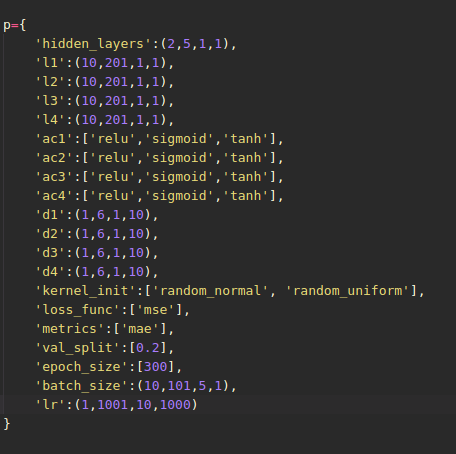
\includegraphics[scale=0.5]{figure/param.png}
    \caption{Hyperparameter search space}
    \label{fig:param_space}
\end{figure}

The hyperparameter search space includes the parameters shown in \ref{fig:param_space}. Tuples represent a range denoted by the notation $\(start,\ end,\ step,\ division\)$. Lists represent specific values that a paramater can take the value of. The function \texttt{rand\textunderscore params()} in \textit{/params.py} produces a random instance of the dictionary, which then can be passed to the Neural Network model for testing. The parameters are explained below.

\\
\begin{itemize}
    \item The hidden layer can be between 2 and 4 layers in length.
    \item Layer $i$ can have $l_{i}$ neurons with range $[10,200]$.
    \item Activation functions can either be $Relu$, $Sigmoid$, or $Tanh$.
    \item Dropout rate of layer $i$ have a range of $[0.1,0.5]$.
    \item Node initialisation can be either Random Normal or Random Uniform.
    \item Batch size can have a range of $[10, 200]$.
    \item Learning rate can have a range of $[0.001, 1]$.
\end{itemize}

Loss, Metric, Validation Split, and Epoch size were kept constant. 

Mean Square Error was chosen as the loss function to reduce loss and punish larger differences between the output and target. Mean Absolute Error was chosen as the metric to monitor progress and since the output is normalised to range $[0,1]$, it is essentially the proportion of error.

\subsubsection{Code Implementation}

Libraries such as $Talos$ exist which work with Keras to implement hyperparameter evaluation, however we decided to write the code for this ourselves.

The algorithm has the following stages: a dictionary of the hyperparameters is created with the name of the hyperparameters as the key, and a possible range of values is passed through. All the elements in the dictionary are then iterated through and a random value for the hyperparameters is selected after which this particular permutation is then ready to be fed into the Neural Network.
\\

\subsubsection{Search for optimal hyperparameters}

As Random Search is used, the number of permutations tried by the algorithm is user decided. To search for the optimal solution, we explored a large number of permutations, and selected a few of the best and further evaluated them. The naive approach to run the algorithm $n$ times was impractical as for large $n$, the program consumes a lot of memory and causes system-wide performance degradation. To circumvent this a bash script was used instead to run call the Python program $n$ times thereby periodically frees up memory. This procedure was left running to produce results for 1000 permutations. 

Once a large set of results was obtained, it was sorted according to the validation metric and pass the top few results for further evaluation using k-fold cross validation.

The model with the optimised hyperparameters are saved into a csv file and sorted by its validation metric (the Mean Absolute Error). We can then used test dataset to evaluate and ensure that the performance is still optimal. the test dataset is only used for final evaluation and not used for selection in parameter search. Finally, the parameters, model architecture, and weights are saved to be used afterwards.

\end{document}
